\chapter{La proprietà intellettuale in campo software}
Dopo aver delineato la sfera della Proprietà Industriale e Intellettuale, si cerca di fare luce sull'attuale sistema di tutela dei diritti che si acquisiscono con la scrittura di un programma per elaboratori; si cerca di cogliere in esso la giusta forma di tutela,  confrontando in particolare realtà diverse della forma di tutela del brevetto in UE e in USA.

\section{Il sistema giuridico delle licenze} \label{sec:sistema-licenze}
Attualmente il software è concepito come espressione dell'intelletto umano, cioè opera dell'ingegno a carattere creativo, e ovviamente ricade nella tutela della Proprietà Intellettuale. Per questo chiunque scrive un programma per elaboratore detiene il cosiddetto copyright, cioè tutti i diritti che si sono evidenziati nel capitolo \ref{cap:uno}.

Si vedrà successivamente come in alcuni casi il diritto d'autore verrà scavalcato dal brevetto nella casistica di brevettazione di un processo fisico che viene associato ad un programma software. \`E stata infatti questa la pratica di molte aziende per iniziare a brevettare il software in via alternativa. Questo aspetto però sarà trattato nelle sezioni successive, dove si farà luce sulla storia della brevettazione software in UE e in USA.

Principalmente il software è prodotto con enormi investimenti per uno scopo molto semplice: l'uso. Negli anni '80 e '90, le software house hanno lucrato su questa rivoluzione digitale fino a diventare multinazionali o comunque colossi dell'informatica.

Si è cercato fin da subito quindi di tutelare il software in maniera tale da avere la possibilità di venderlo, pur rimanendo sempre i proprietari. Come si sa su di esso si possiede il diritto d'autore (cioè la proprietà intellettuale, non la proprietà del supporto con cui viene venduto) ed è proprio su questa facoltà che è nato il contratto tra un licenziatario \footnote{colui che ne detiene il copyright e ne cede alcuni in cambio di denaro o altro} e un licenziante \footnote{qualsiasi utente dell'opera}. Questo accordo scritto prende comunemente il nome di licenza.

Nel particolare la licenza segue il modello uno a molti tra licenziante e licenziatario e si definisce con il termine ``contratto di licenza''. La parola contratto deriva dal modo di tutelare la trasmissione dei diritti d'autore cioè nel senso classico di accordo  tra due o più parti per costituire, regolare o estinguere un rapporto giuridico patrimoniale”.
Il termine licenza invece si definisce come un atto unilaterale giuridico, originario del diritto amministrativo, con cui un soggetto concede un'autorizzazione a compiere una determinata attività. \`E importante sottolineare come l'uso del vocabolo ``licenza'' derivi dal termine coniato negli States e tradotto letteralmente da \textit{mass market licenses of copyright material }.

In sintesi quindi l'obietto che si prefigge una licenza riguarda cessione di alcuni diritti come, ad esempio, il diritto all'uso: infatti con l'acquisto di un software, e la conseguente sottoscrittura alla licenza, non si compra il software in sè, inalienabile dall'autore, ma il diritto all'uso e in alcuni casi (come nel copyleft) anche il diritto alla modifica e alla copia/ridistribuzione.

In questa sezione si è visto come inizialmente in tutte le legislazione l'idea di software coincida con un'opera logico-matematica tutelabile da diritto d'autore e quindi appartenente alla sfera della Proprietà Intellettuale. Ovviamente poi si è reso necessario una forma più stringente e tagliente di tutela che in qualche modo poteva tutelare le lobby del software anche dalla possibile minaccia di copia tra sè stesse, visti la particolare natura immateriale/virtuale del software e il boom industriale legato al suo commercio.

Questo atteggiamento è ampiamente attecchito ``de facto'' in America e invece meno ratificato in Europa in quanto il dibattito risulta ancora acceso anche da un punto di vista politico.

\section{La situazione dell'UE sui brevetti software}
La situazione europea e mondiale sulla questione dei brevetti software è molto spinosa, in quanto risulta molto complesso delimitare i confini per cui il software inteso come esclusivo codice possa ritenersi brevettabile oppure una invenzione tecnica basata su software possa ritenersi non brevettabile.

Da quando è in vigore (anni '70) la Convenzione europea dei Brevetti all'interno dell'Unione Europea l'Organizzazione Europea dei Brevetti ha rilasciato molti brevetti su invenzioni basate almeno in parte su software; questo è in parte in controtendenza con il comportamento sempre avuto dal vecchio continente, da dove (per la precisione in Francia) nel 1968\cite{invenzione-software}, è nata la prima norma in materia brevettuale tesa ad escludere dalla tutela i programmi per elaboratore.

L'articolo 52  della convenzione esclude esplicitamente i programmi per computer dalla brevettabilità (comma 2), intesi come programmi per computer in quanto tali (comma 3). L'interpretazione data all'articolo è che ogni invenzione che offre un contributo tecnico non ovvio o risolve problemi tecnici in maniera non banale sia brevettabile anche se comprende una parte software.

Ovviamente non può essere sufficiente affidare l'intera legislazione di un settore così importante a livello scientifico ed economico ad una mera distinzione di carattere semantico, ma deve essere approfondito l'ambito di utilizzo e di realizzazione del software stesso.

Prima di tutto è da notare che è impossibile che il legislatore abbia impiegato la definizione ``programmi in quanto tali'' riferendosi esclusivamente alla forma codificata delle informazioni, lasciando brevettabili tutti i processi che le istruzioni producono, in quanto il software è stato incluso nella categoria delle opere non brevettabili come ``attività intellettuale'' e non come ``presentazione di informazioni''.

Per inquadrare correttamente il software all'interno della disciplina brevettuale occorre prenderlo in considerazione in due momenti: innanzitutto come registrato su un supporto di memorizzazione (inteso quindi come insieme di informazioni, sequenza di istruzioni), in secondo luogo all'atto dell'esecuzione, quando tramite le istruzioni va a regolare il comportamento della macchina.

Il primo momento dei due appena descritti è stabilmente appartenente all'area del non-brevettabile, essendo il funzionamento del supporto completamente indipendente da ciò che ne viene memorizzato sopra, ed essendo totalmente libero il genere di informazioni che possono essere registrate sul supporto. Ristretto a questo momento il concetto di software è riconducibile alle ``presentazioni di informazioni'', escluse dalla brevettabilità con chiarezza (articoli 52 n.2 lett.\textit{d} CBE e 12 co.2 lett.\textit{c} l.i.).

Il momento di interesse alla trattazione è quello che riguarda il funzionamento del software all'interno dell'elaboratore, in quanto si realizza lo scopo pratico per cui il software è stato scritto.

La tesi che supporta la non brevettabilità del software appoggiandosi alla separazione fisica tra software ed hardware, attribuisce totale indipendenza alla funzionalità del software in riferimento allo specifico hardware su cui viene eseguito. Una procedura, idealmente, può essere eseguita su qualsiasi tipo di computer implicando quindi che lo sforzo mentale che ha portato all'invenzione della procedura prescinda dalla macchina sulla quale poi sarà implementata.

L'hardware non può essere quindi considerato come parte integrante dell'invenzione; la presenza di questo nell'esecuzione del software (nonostante sia composto da tutti componenti brevettabili) non è sufficiente a sancire la brevettabilità del software.

Esiste anche una ricostruzione più rigida, sempre a favore della non-brevettabilità del software e di matrice più dogmatico/filosofica, nata in Germania prima che il paese si adattasse alla convenzione di Monaco. In questa ricostruzione l'attenzione è spostata a livello ``ontologico'' sulla differenza che intercorre tra il concetto di ``invenzione brevettabile'' e ``algoritmo''. \`E da precisare che, nonostante questa interpretazione ormai superata dalla convenzione di Monaco a livello temporale, è tuttora ritenuta il fondamento della non brevettabilità del software in Europa, e viene citata come fonte ideologica di questa scelta.

In Germania è ormai una definizione classica di ``invenzione brevettabile'' un qualcosa che insegni ad utilizzare le forze naturali, fatto eccetto di quelle che regolano l'attività mentale, con il fine di ottenere un nuovo risultato tangibile direttamente attraverso il dominio dei rapporti causali relativi a tali forze.

L'algoritmo invece è concepito come una procedura astratta per la soluzione di un problema, la cui validità e risultato prescindono dall'impiego diretto delle forze della natura; l'uso di mezzi materiali è quindi successivo al completamento dell'idea inventiva, in quanto riguarda solamente una sua possibile attuazione.

Per cui emerge da questa teoria che il problema di carattere tecnico riguardante la realizzazione dell'hardware in grado di svolgere le operazioni richieste dal software è indiscutibilmente appartenente alla categoria del ``brevettabile'' mentre il problema concernente la procedura logico-matematica che poi dovrà essere attuata meccanicamente dalla macchina si risolve prima di entrare nella sfera del mondo fisico, in quanto i risultati sono costanti e ripetibili indipendentemente, e possono essere dimostrati anche su un piano meramente astratto.

Su questa base, l'attività del programmatore di tradurre (successivamente alla concezione logica della procedura) l'algoritmo in un concreto software non aggiunge niente al concetto espresso dall'invenzione dell'algoritmo; è come se il programmatore eseguisse un'attività compilativa, all'interno di confini già tracciati dall'invenzione della procedura algoritmica. La stesura del software quindi si concentra nello sfruttare la macchina secondo il suo scopo.

La conclusione di questo pensiero porta quindi a evidenziare che nell'invenzione di software è assente l'utilizzo diretto delle forze della natura, in quanto l'impiego dei mezzi fisici non è collegato causalmente all'attività inventiva. I mezzi fisici intervengono solamente al termine del processo inventivo, ovvero al momento della trasformazione dell'algoritmo in programma, confermando pertanto la non brevettabilità di questo.

All'interno dell'Unione Europea finora è riuscito a rimanere saldo questo principio, riconosciuto anche dal Parlamento Europeo stesso in più momenti. Il più importante di questi è stato probabilmente il 24 settembre 2003, dove è stata riconosciuta la separazione del software dal contesto tecnico e ne è stata limitata la brevettabilità; l'atto tecnico è stata l'approvazione in prima lettura della Direttiva Europea n.2002/47 con l'apporto (rispetto al provvedimento originario del 2002) di numerosi e fondamentali emendamenti che confermano il divieto di brevettazione del software .

Nonostante la pressione di molte \textit{lobby} del settore informatico, che hanno indotto il Consiglio dell'Unione Europea in primis (18 maggio 2004) e la Presidenza dell'Unione Europea in seconda battuta (7 marzo 2005) a tentare di ribaltare, tramite una direttiva, la decisione parlamentare a favore della non brevettazione del software, il 6 luglio 2005 con 648 voti favorevoli, 14 contrari e 18 astenuti, il Parlamento Europeo ha ripristinato quanto legiferato nel 2003, bocciando in seconda lettura tale direttiva e riconoscendo la non brevettabilità del software all'interno dell'Unione Europea.

\section{I brevetti software in USA}

Molto diversa e ben più decisa nelle scelte (almeno apparentemente) dalla situazione europea, appare la gestione dei brevetti software negli Stati Uniti. Questa è da mettere in luce in quanto è il paese che detiene, secondo i dati forniti dal USA Paten Office, circa il 60\% del mercato mondiale del software.

Innanzitutto anche negli States si ebbe l'echeggiare della prima interpretazione data alla brevettabilità del software: la concezione tedesca dell'assenza di carattere tecnico dei programmi, considerandoli alla stregua di \textit{mental steps} non brevettabili. Questa concezione incontrò infatti nei primi anni '60 l'appoggio del Patent Office. Questo orientamento però incontrò tuttavia una radicale opposizione da parte della giurisprudenza della \textit{Court of Costum and Patent Appeal}, fintantochè non si arrivò negli anni '70 a non considerare più programmi per elaboratori come meri algoritmi matematici.

Più nel dettaglio il caso più emblematico di questa concezione derivante dalla Germania, fu il primo caso in cui il problema della brevettabilità del software venne esaminato: fu il caso denominato ``Gottschalk v. Benson'' in cui, nel 1972, la Corte Suprema si occupò della possibilità di brevettare un programma per elaboratore consistente in un metodo di conversione di un sistema decimale codificato in binario in un sistema binario puro mediante l'uso di un algoritmo. La conversione poteva essere effettuata anche a mano, ma l'algoritmo consentiva di farla effettuare ad un elaboratore in modo da risparmiare tempo ed energie. La Corte Suprema si affermò contraria alla brevettabilità del richiesto algoritmo ritenendo il processo di conversione sopra citato un vero e proprio algoritmo, ossia una procedura per la soluzione di un problema matematico che, in quanto tale, non è brevettabile. Ciò per evitare il crearsi di un diritto di monopolio su una formula matematica, su un concetto o su un modo di pensare che devono essere lasciati al libero sfruttamento di chiunque e che, per definizione, non poteva essere messo sotto brevetto.

Mentre le richieste di brevetto pervenivano sempre più numerose, la prima decisione con la quale la Corte Suprema sanzionò la validità di un brevetto concernente un programma per elaboratore, fu con il successivo e fondamentale caso denominato ``Diamond v. Diehr'' del 1981. In questo caso la Corte Suprema stabilì che l'ufficio brevetti doveva concedere un brevetto, anche se una parte importante dell'invenzione consisteva in un programma per elaboratori che utilizzava formule già note: la Corte Suprema affermò che in questo caso l'invenzione non era un mero algoritmo matematico, ma un processo per fondere la gomma, quindi brevettabile. Tecnicamente si brevettava un software utilizzato nel processo di stampaggio degli oggetti di gomma che consentiva di controllare ripetutamente la temperatura all'interno dello stampo e calcolare il tempo ottimale di formatura, trascorso il quale il programma comandava l'apertura dello stampo medesimo.

In seguito e questo evento furono concessi altri brevetti su software anche se con risultati contrastanti e confusi. Questo perché iniziò a decadere quella valenza logico matematica che aveva caratterizzato negli anni 50-60 l'Ufficio Brevetti. In particolare ``mental step doctrine'' cadde per i seguenti motivi:

\begin{itemize}
	\item si distinse tra processi/passi mentali e steps eseguiti meccanicamente da un dispositivo fisico come un calcolare.
	\item si differenziò l'indeterminatezza della logica umana dalla determinatezza delle macchina
	\item Si osservò che una dispositivo fisico è composto da hardware e software e che quest'ultimo può cambiare il comportamento del dispositivo fisico
\end{itemize}
In questo senso queste obiezioni misero in luce gli aspetti che distinguono i programmi per elaboratore dalle creazioni tradizionali escluse dalla brevettazione, mettendo sempre più in evidenza una sostanziale unione tra hardware e software, contrariamente al dibattito dell'Europa e  diversamente dalla visione tedesca in cui il software si riduce all'esecuzione, secondo modalità prestabilite, di una procedura in sè già completa indipendentemente dai mezzi in cui è svolta.

In USA poi la Corte d'Appello del Circuito Federale tolse ogni dubbio attraverso una serie di regolamentazioni che inquadravano il software eseguito su una macchina come un dispositivo fisico. La prima denominata \textit{In re Alappat} afferma che un nuovo algoritmo abbinato ad un'elementare componente fisica costituisce un nuovo dispositivo fisico. Ne consegue che un calcolatore su cui è caricato un algoritmo originale diventa una ``nuova macchina'', brevettabile secondo le tradizionali normative statunitensi sul software. Ciò venne ulteriormente sostenuta da una seconda norma \textit{In re Lowry} che affermava che le strutture di dati rappresentanti l'informazione contenute in un disco fisso o una memoria deve essere similmente considerata come un dispositivo fisico.

In conclusione negli anni '90 ci fu la svolta definitiva a favore dei brevetti: attraverso la nomina di Bruce Lehman commissario dell'ufficio brevetti e marchi, il quale non era un avvocato specializzato in brevetti ma uno dei principali lobbisti dell'industria del software; nel 1995 l'ufficio stabilì alcune linee guida per l'esame e la registrazione di brevetti software, diventando così senza una piena decisione, apparentemente validi.

In sintesi dalla travagliata storia Americana, è pacifico ormai che non si possa escludere la brevettabilità un processo solo perché si contiene un software;e d'altro canto, non è sufficiente dire che l'invenzione si sostanzia in un algoritmo per rigettare la domanda di brevetto. Ancora, non è vero che un'invenzione non può essere brevettata perché il procedimento è eseguito da un elaboratore e è descritta sotto forma di un programma elettronico. Vista la sostanziale affinità tra algoritmi matematici e software, sarà ritenuto brevettabile quel software che non si esaurisca in alcuna formula o algoritmo matematico, ma si concretizzi, al contrario, in un'applicazione pratica.

Su questa linea si è messo a punto un criterio basato su un duplice accertamento \textit{(two steps doctrine)} per poter distinguere i programmi brevettabili da quelli non brevettabili. Per quanto riguarda il primo accertamento la Corte \textit{(Court of Customs and Patent Appeals)} afferma che occorre distinguere tra un concetto di algoritmo più ampio ed uno più ristretto. Il primo comprende quei procedimenti in cui la successione delle attività necessarie per realizzare un determinato fine è descritta passo dopo passo \footnote{a step-by-step procedure for solving a problem or accomplishing some end}; il secondo comprende soltanto quei procedimenti volti a risolvere un problema matematico.




\begin{figure}[bh]
	\begin{center}
		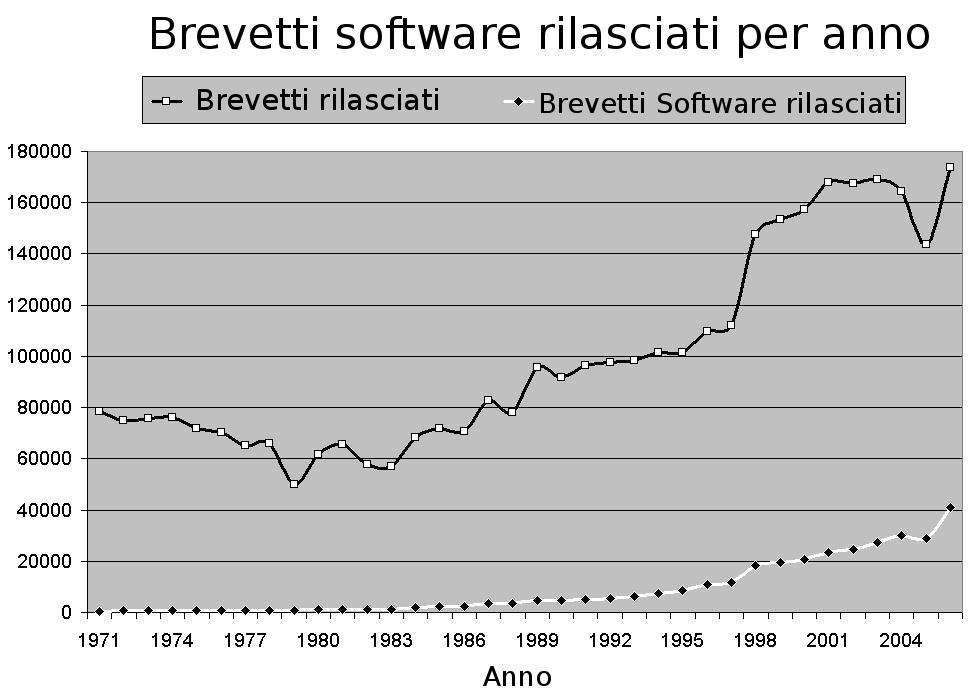
\includegraphics[scale=0.55]{figure/UsPatent.png}
	\end{center}
	\caption{\textit{Nel grafico è possibile notare la crescita dei brevetti rispetto a quelli software nel mercato USA}}
\end{figure}

